%!TeX root=../tempestrackham.tex

\Act*{5}
\Scene*{1}[Before \textsc{Prospero's} cell.]

\begin{figure}[t]
	\centering
	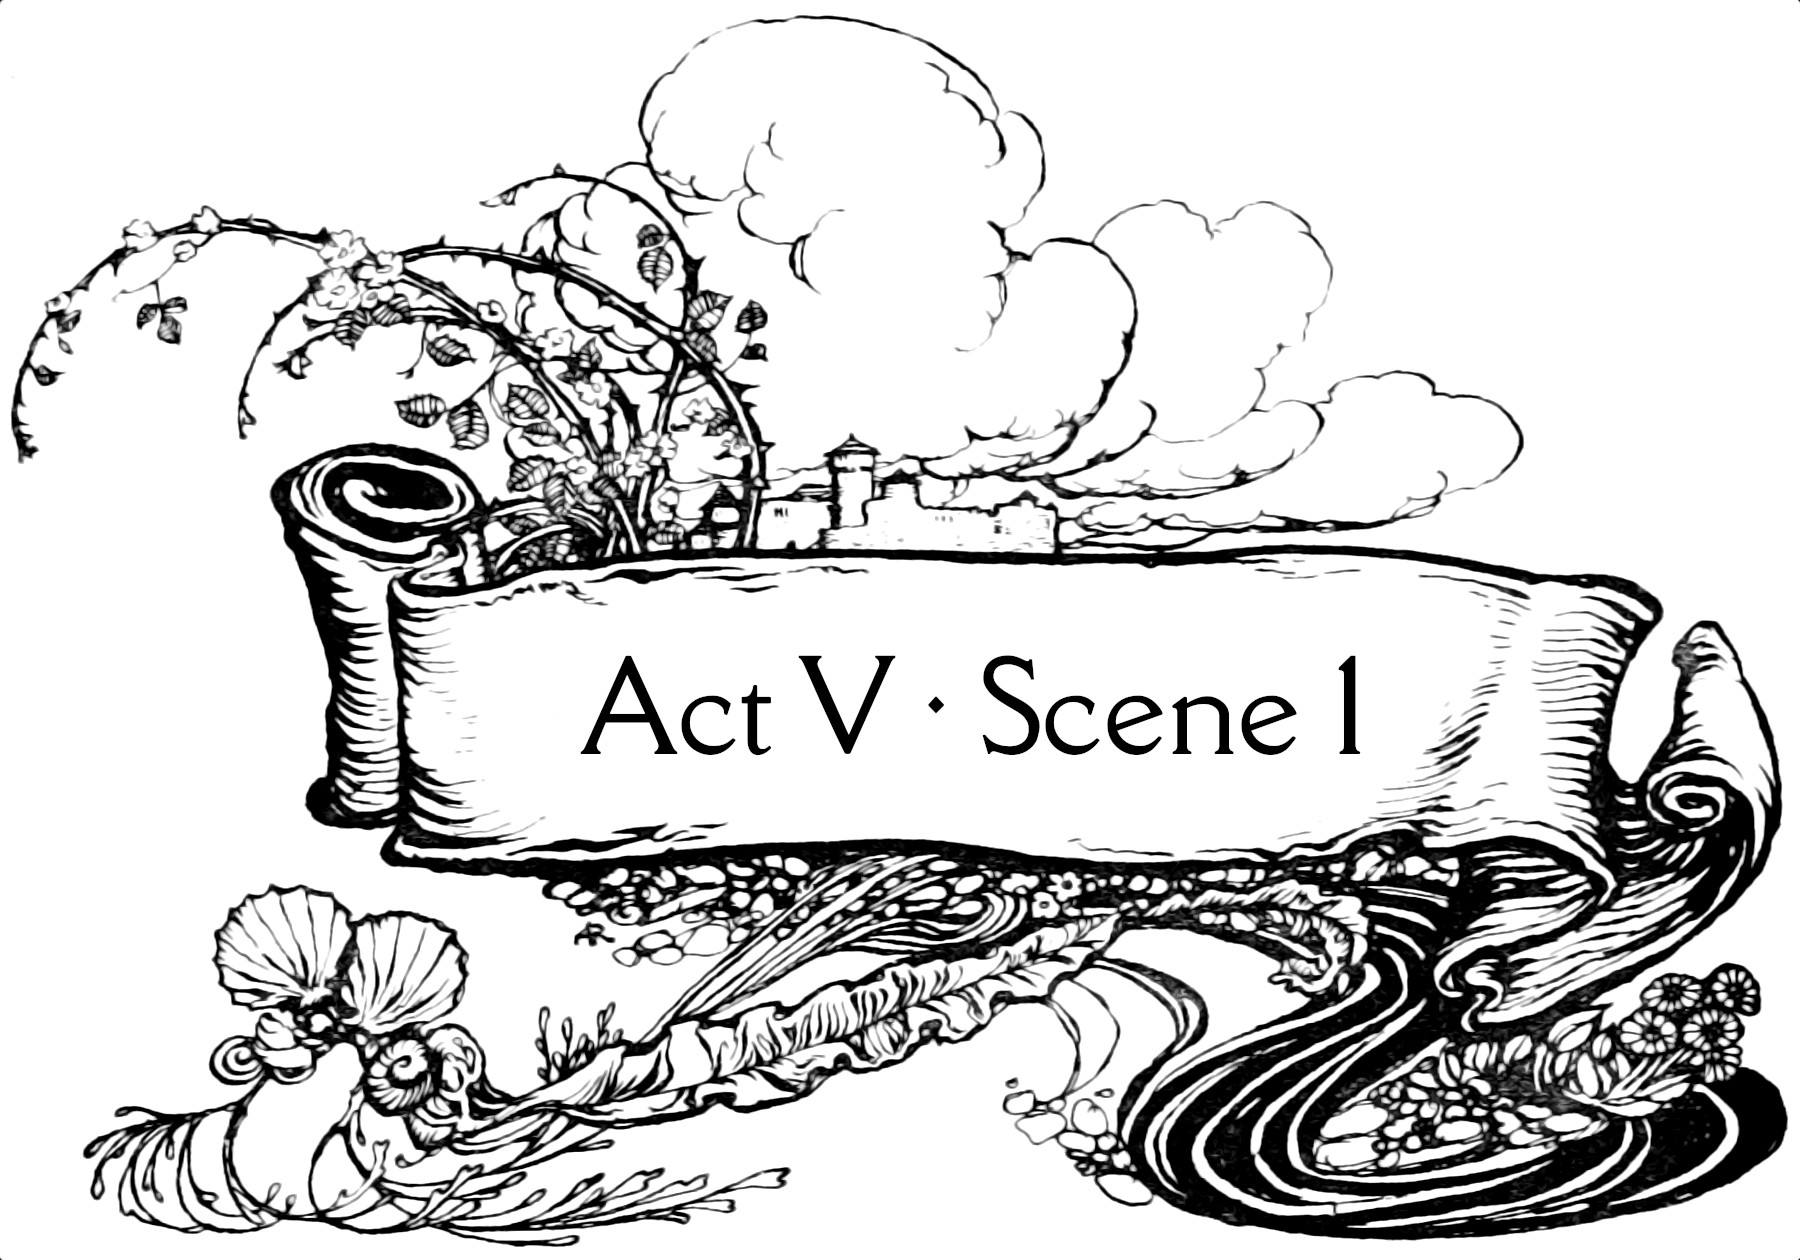
\includegraphics[width=\headerwidth]{5ihead}
\end{figure}

\vspace{\textsink}

\textit{(Before \textsc{Prospero's} cell.)}\centering

\enter{\textsc{Prospero} in his magic robes, and \textsc{Ariel}}

\begin{verse_speech}[Prospero] 
Now does my project gather to a head:\\
My charms crack not; my spirits obey; and time\\
Goes upright with his carriage. How's the day?
\end{verse_speech}

\begin{verse_speech}[Ariel] 
On the sixth hour; at which time, my lord,\\
You said our work should cease.
\end{verse_speech}

\begin{verse_speech}[Prospero] 
\hspace{\widthof{You said our work should cease.}}I did say so,\\
When first I raised the tempest. Say, my spirit,\\
How fares the king and's followers?
\end{verse_speech}

\begin{verse_speech}[Ariel] 
\hspace{\widthof{How fares the king and's followers?}}Confined together\\
In the same fashion as you gave in charge,\\
Just as you left them; all prisoners, sir,\\
In the line-grove which weather-fends your cell;\\
They cannot budge till your release. The king,\\
His brother and yours, abide all three distracted\\
And the remainder mourning over them,\\
Brimful of sorrow and dismay; but chiefly\\
Him that you term'd, sir, <The good old lord Gonzalo;>\\
His tears run down his beard, like winter's drops\\
From eaves of reeds. Your charm so strongly works 'em\\
That if you now beheld them, your affections\\
Would become tender.
\end{verse_speech}

\verseline[Prospero]{\hspace{\widthof{Would become tender.}}Dost thou think so, spirit?}

\verseline[Ariel]{Mine would, sir, were I human.}

\begin{verse_speech}[Prospero] 
\hspace{\widthof{Mine would, sir, were I human.}}And mine shall.\\
Hast thou, which art but air, a touch, a feeling\\
Of their afflictions, and shall not myself,\\
One of their kind, that relish all as sharply,\\
Passion as they, be kindlier moved than thou art?\\
Though with their high wrongs I am struck to the quick,\\
Yet with my nobler reason 'gainst my fury\\
Do I take part: the rarer action is\\
In virtue than in vengeance: they being penitent,\\
The sole drift of my purpose doth extend\\
Not a frown further. Go release them, Ariel:\\
My charms I'll break, their senses I'll restore,\\
And they shall be themselves.
\end{verse_speech}

\verseline[Ariel]{\hspace{\widthof{And they shall be themselves.}}I'll fetch them, sir.}
	
\exit{Ariel}

\stage{\textsc{Prospero} draws a large circle on the stage with his staff.}

\begin{verse_speech}[Prospero] 
Ye elves of hills, brooks, standing lakes and groves,\\
And ye that on the sands with printless foot\\
Do chase the ebbing Neptune and do fly him\\
When he comes back; you demi-puppets that\\
By moonshine do the green sour ringlets make,\\
Whereof the ewe not bites, and you whose pastime\\
Is to make midnight mushrooms, that rejoice\\
To hear the solemn curfew; by whose aid,\\
Weak masters though ye be, I have bedimm'd\\
The noontide sun, call'd forth the mutinous winds,\\
And 'twixt the green sea and the azured vault\\
Set roaring war: to the dread rattling thunder\\
Have I given fire and rifted Jove's stout oak\\
With his own bolt; the strong-based promontory\\
Have I made shake and by the spurs pluck'd up\\
The pine and cedar: graves at my command\\
Have waked their sleepers, oped, and let 'em forth\\
By my so potent art. But this rough magic\\
I here abjure, and, when I have required\\
Some heavenly music, which even now I do,\\

\stage{He gestures with his staff}

To work mine end upon their senses that\\
This airy charm is for, I'll break my staff,\\
Bury it certain fathoms in the earth,\\
And deeper than did ever plummet sound\\
I'll drown my book.
\end{verse_speech}

\stage{Solemn music}

\stage{Re-enter \textsc{Ariel} before: then \textsc{Alonso}, with a frantic gesture, attended by \textsc{Gonzalo}; \textsc{Sebastian} and \textsc{Antonio} in like manner, attended by \textsc{Adrian} and \textsc{Francisco} they all enter the circle which \textsc{Prospero} had made, and there stand charmed; which \textsc{Prospero} observing, speaks:}

\begin{verse_speech}[Prospero] 
A solemn air and the best comforter\\
To an unsettled fancy cure thy brains,\\
Now useless, boil'd within thy skull! There stand,\\
For you are spell-stopp'd.\\
Holy Gonzalo, honourable man,\\
Mine eyes, even sociable to the show of thine,\\
Fall fellowly drops. The charm dissolves apace,\\
And as the morning steals upon the night,\\
Melting the darkness, so their rising senses\\
Begin to chase the ignorant fumes that mantle\\
Their clearer reason. O good Gonzalo,\\
My true preserver, and a loyal sir\\
To him you follow'st! I will pay thy graces\\
Home both in word and deed. Most cruelly\\
Didst thou, Alonso, use me and my daughter:\\
Thy brother was a furtherer in the act.\\
Thou art pinch'd fort now, Sebastian. Flesh and blood,\\
You, brother mine, that entertain'd ambition,\\
Expell'd remorse and nature; who, with Sebastian,\\
Whose inward pinches therefore are most strong,\\
Would here have kill'd your king; I do forgive thee,\\
Unnatural though thou art. Their understanding\\
Begins to swell, and the approaching tide\\
Will shortly fill the reasonable shore\\
That now lies foul and muddy. Not one of them\\
That yet looks on me, or would know me Ariel,\\
Fetch me the hat and rapier in my cell.\\

\stage{\textsc{Ariel} exits and at once returns with \textsc{Prospero’s} ducal robes.}

I will discase me, and myself present\\
As I was sometime Milan: quickly, spirit;\\
Thou shalt ere long be free.
\end{verse_speech}

\stage{\textsc{Ariel} sings and helps to attire him}
\begin{song}
\songline{Where the bee sucks. there suck I:}
\songline{In a cowslip's bell I lie;}
\songline{There I couch when owls do cry.}
\songline{On the bat's back I do fly}
\songline{After summer merrily.}
\songline{\hspace{1em} Merrily, merrily shall I live now}
\songline{Under the blossom that hangs on the bough.}
\end{song}

\begin{verse_speech}[Prospero] 
Why, that's my dainty Ariel! I shall miss thee:\\
But yet thou shalt have freedom: so, so, so.\\
To the king's ship, invisible as thou art:\\
There shalt thou find the mariners asleep\\
Under the hatches; the master and the boatswain\\
Being awake, enforce them to this place,\\
And presently, I prithee.
\end{verse_speech}

\begin{verse_speech}[Ariel] 
I drink the air before me, and return\\
Or ere your pulse twice beat.
\end{verse_speech}

\exit{Ariel}

\begin{pictures} % Merrily
	\begin{letter}
		\begin{colorbigpic}
			[1.1]
			{5i_merrily}
			{Merrily, merrily shall I live now}
		\end{colorbigpic}
	\end{letter}
	\begin{a4}
		\begin{colorbigpic}
			[1]
			{5i_merrily}
			{Merrily, merrily shall I live now}
		\end{colorbigpic}
	\end{a4}
\end{pictures}

\begin{verse_speech}[Gonzalo] 
All torment, trouble, wonder and amazement\\
Inhabits here: some heavenly power guide us\\
Out of this fearful country!
\end{verse_speech}

\begin{verse_speech}[Prospero] 
\textit{(To \textsc{Alonso})}\hspace{\widthof{Out of this fearful country!}-\widthof{(To \textsc{Alonso})}}Behold, sir king,\\
The wrongèd Duke of Milan, Prospero:\\
For more assurance that a living prince\\
Does now speak to thee, I embrace thy body;\\

\stage{He embraces \textsc{Alonso}}

And to thee and thy company I bid\\
A hearty welcome.
\end{verse_speech}

\begin{verse_speech}[Alonso] 
\hspace{\widthof{A hearty welcome.}}Whether thou best he or no,\\
Or some enchanted trifle to abuse me,\\
As late I have been, I not know: thy pulse\\
Beats as of flesh and blood; and, since I saw thee,\\
The affliction of my mind amends, with which,\\
I fear, a madness held me: this must crave,\\
An if this be at all, a most strange story.\\
Thy dukedom I resign and do entreat\\
Thou pardon me my wrongs. But how should Prospero\\
Be living and be here?
\end{verse_speech}

\begin{verse_speech}[Prospero] 
\textit{(To \textsc{Gonzalo})}\hspace{\widthof{Be living and be here?}-\widthof{(To Gonzalo)}}First, noble friend,\\
Let me embrace thine age, whose honour cannot\\
Be measured or confined.
\end{verse_speech}

\begin{verse_speech}[Gonzalo] 
\hspace{\widthof{Be measured or confined.}}Whether this be\\
Or be not, I'll not swear.
\end{verse_speech}



\begin{verse_speech}[Prospero] 
\hspace{\widthof{Or be not, I'll not swear.}}You do yet taste\\
Some subtilties o' the isle, that will not let you\\
Believe things certain. Welcome, my friends all!\\
\asideto{Sebastian and Antonio}{But you, my brace of lords, were I so minded,\\
I here could pluck his highness' frown upon you\\
And justify you traitors: at this time\\
I will tell no tales.}
\end{verse_speech}

\verseline[Sebastian]{\aside{The devil speaks in him.}}

\begin{verse_speech}[Prospero] 
\asideto{Sebastian}{No.}\\
\textit{(To \textsc{Antonio})} For you, most wicked sir, whom to call brother\\
Would even infect my mouth, I do forgive\\
Thy rankest fault; all of them; and require\\
My dukedom of thee, which perforce, I know,\\
Thou must restore.
\end{verse_speech}

\begin{verse_speech}[Alonso] 
\hspace{\widthof{Thou must restore.}}If thou be'st Prospero,\\
Give us particulars of thy preservation;\\
How thou hast met us here, who three hours since\\
Were wreck'd upon this shore; where I have lost—\\
How sharp the point of this remembrance is!—\\
My dear son Ferdinand.
\end{verse_speech}

\verseline[Prospero]{\hspace{\widthof{My dear son Ferdinand.}}I am woe for't, sir.}

\begin{verse_speech}[Alonso] 
Irreparable is the loss, and patience\\
Says it is past her cure.
\end{verse_speech}

\begin{verse_speech}[Prospero] 
\hspace{\widthof{Says it is past her cure.}}I rather think\\
You have not sought her help, of whose soft grace\\
For the like loss I have her sovereign aid\\
And rest myself content.
\end{verse_speech}

\verseline[Alonso]{\hspace{\widthof{And rest myself content.}}You the like loss?}

\begin{verse_speech}[Prospero] 
As great to me as late; and, supportable\\
To make the dear loss, have I means much weaker\\
Than you may call to comfort you, for I\\
Have lost my daughter.
\end{verse_speech}

\begin{verse_speech}[Alonso] 
A daughter?\\
O heavens, that they were living both in Naples,\\
The king and queen there! that they were, I wish\\
Myself were mudded in that oozy bed\\
Where my son lies. When did you lose your daughter?
\end{verse_speech}

\begin{verse_speech}[Prospero] 
In this last tempest. I perceive these lords\\
At this encounter do so much admire\\
That they devour their reason and scarce think\\
Their eyes do offices of truth, their words\\
Are natural breath: but, howsoe'er you have\\
Been justled from your senses, know for certain\\
That I am Prospero and that very duke\\
Which was thrust forth of Milan, who most strangely\\
Upon this shore, where you were wreck'd, was landed,\\
To be the lord on't. No more yet of this;\\
For 'tis a chronicle of day by day,\\
Not a relation for a breakfast nor\\
Befitting this first meeting. \textit{(To \textsc{Alonso})} Welcome, sir;\\
This cell's my court: here have I few attendants\\
And subjects none abroad: pray you, look in.\\
My dukedom since you have given me again,\\
I will requite you with as good a thing;\\
At least bring forth a wonder, to content ye\\
As much as me my dukedom.
\end{verse_speech}

\stage{Here \textsc{Prospero} discovers \textsc{Ferdinand} and \textsc{Miranda} playing at chess}

\verseline[Miranda]{Sweet lord, you play me false.}

\begin{verse_speech}[Ferdinand] 
\hspace{\widthof{Sweet lord, you play me false.}}No, my dear'st love,\\
I would not for the world.
\end{verse_speech}

\begin{verse_speech}[Miranda] 
Yes, for a score of kingdoms you should wrangle,\\
And I would call it fair play.
\end{verse_speech}

\begin{verse_speech}[Alonso] 
\hspace{\widthof{And I would call it fair play.}}If this prove\\
A vision of the Island, one dear son\\
Shall I twice lose.
\end{verse_speech}

\verseline[Sebastian]{\hspace{\widthof{Shall I twice lose.}}A most high miracle!}


\begin{pictures} % Ringlets - letter
	\begin{letter}
		% \clearpage
		% \begin{tikzpicture}[remember picture, overlay]
			% \node (img) at ($(current page.center)+(0cm,0.5cm)$) {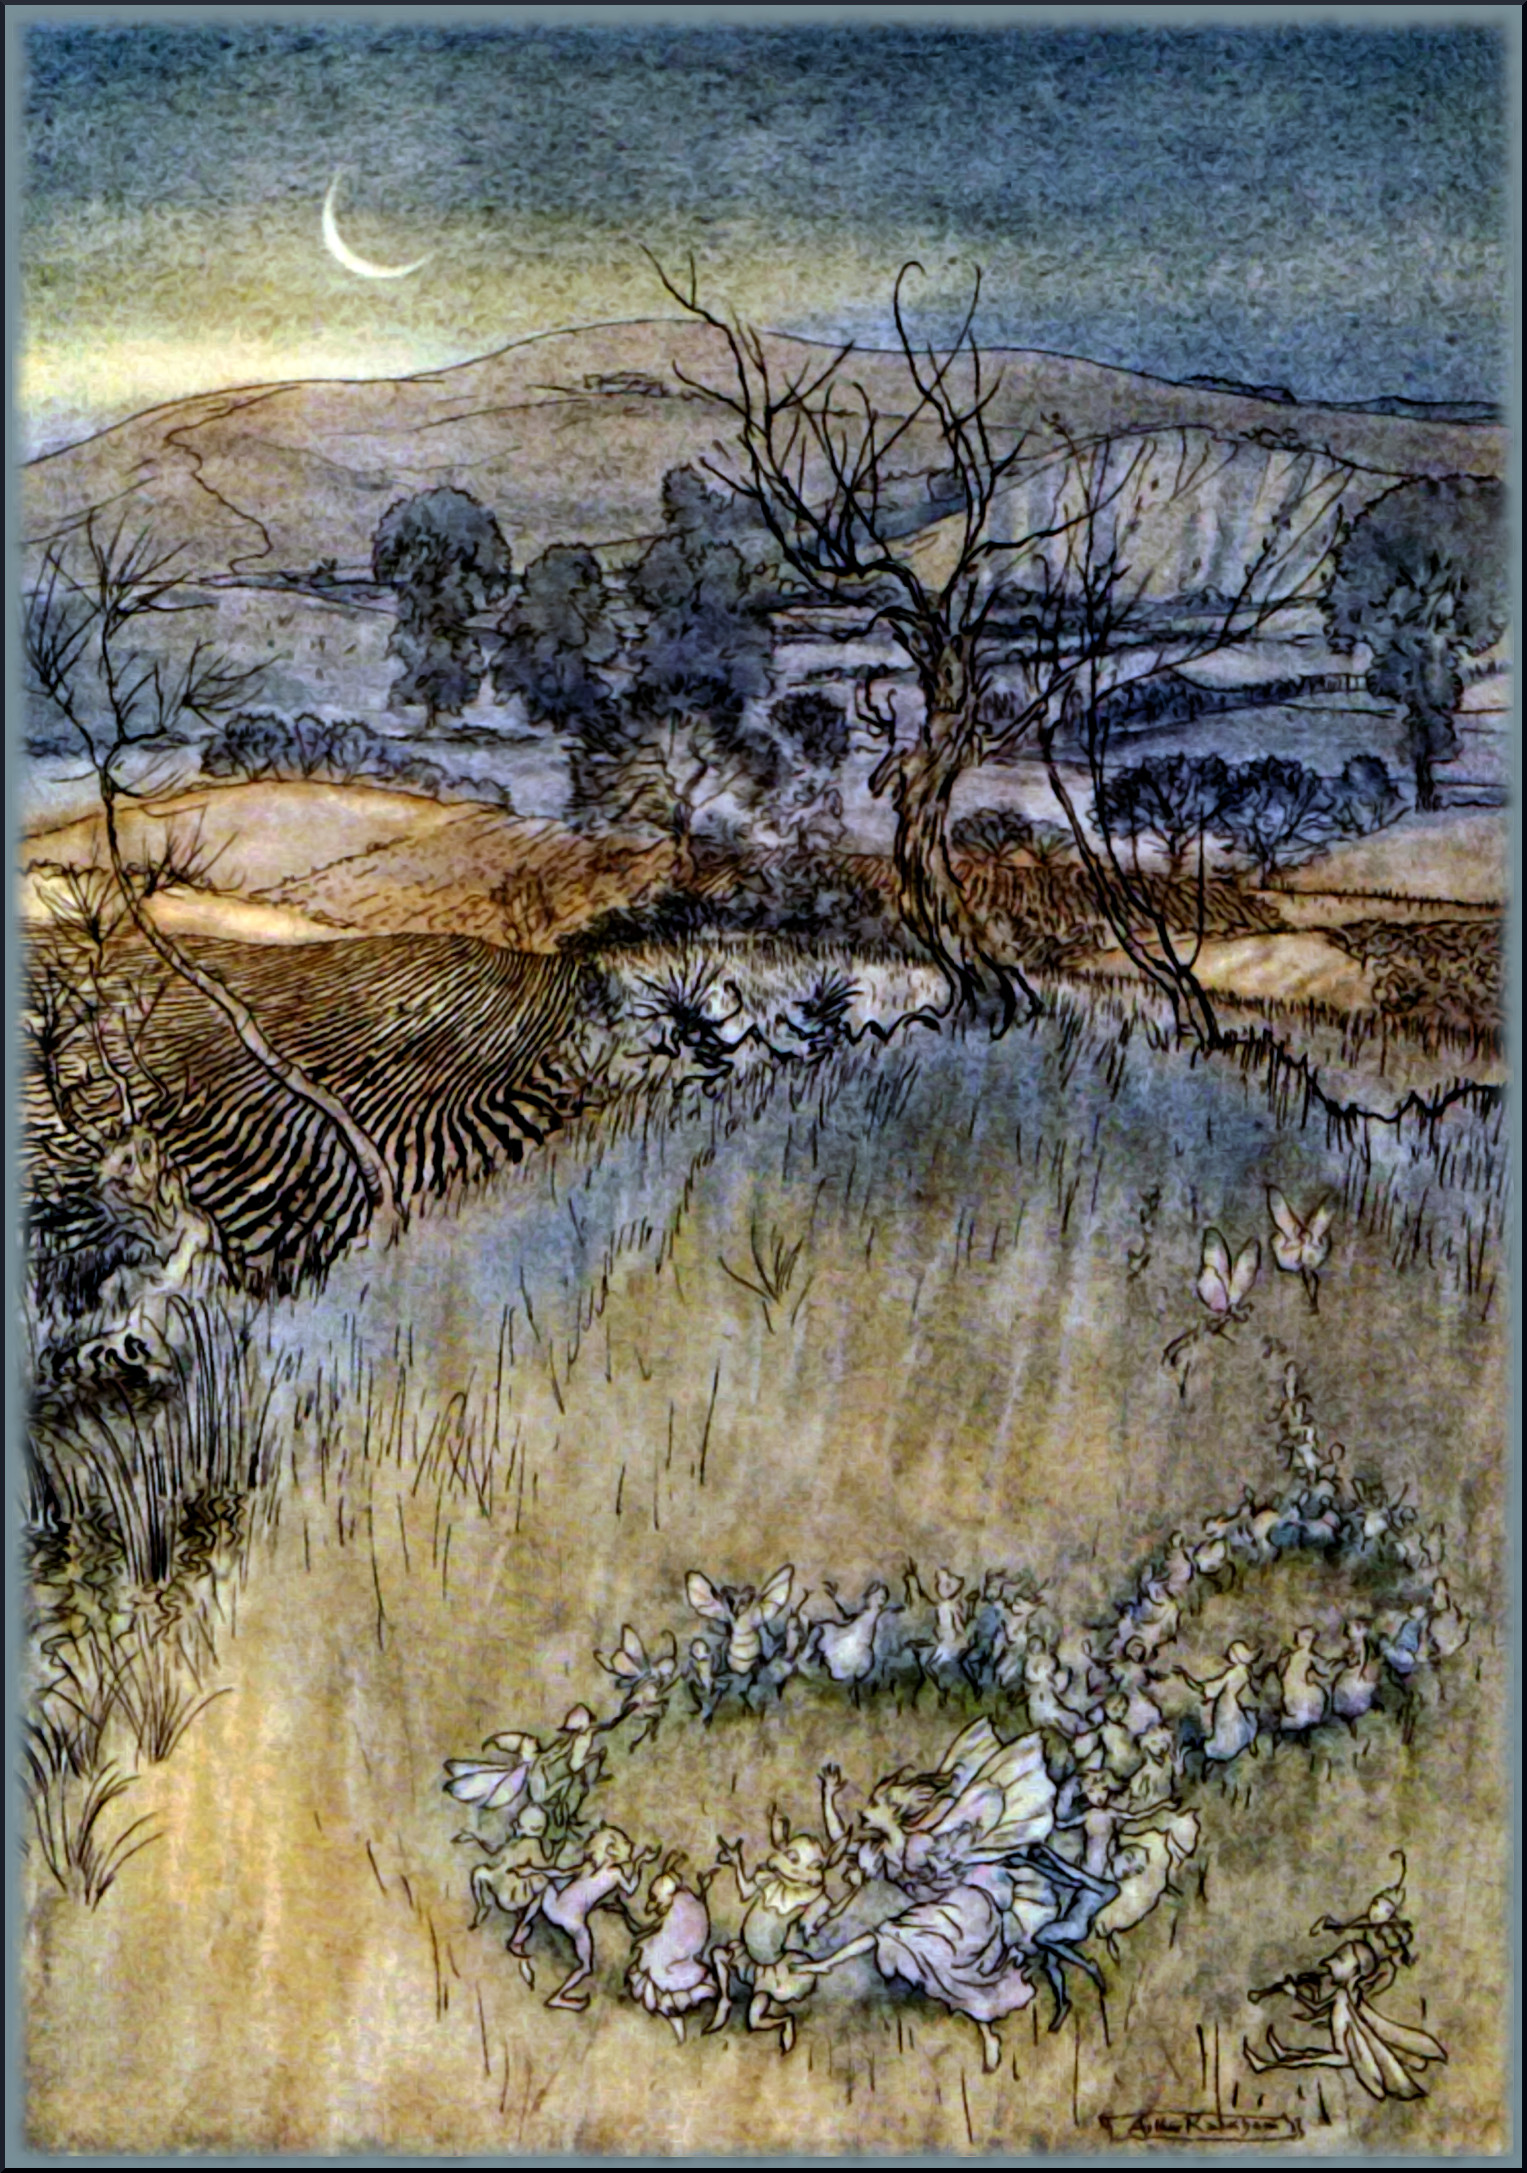
\includegraphics[width=\coverwidth]{5i_ringlets}};
			% \node[text width=0.9\textwidth, align=center] (caption) at ($(current page.south)+(0cm,2cm)$) {\textsc{Ye elves of hills... that by moonshine do... ringlets make}};
		% \end{tikzpicture}
		% \thispagestyle{empty}
		% \clearpage
		\begin{colorbigpic}
			[1.1]
			{5i_ringlets}
			{Ye elves of hills\dots that by moonshine do\dots ringlets make}
		\end{colorbigpic}
	\end{letter}
\end{pictures}

\begin{verse_speech}[Ferdinand] 
	\textit{(seeing \textsc{Alonso} and coming forward)}
Though the seas threaten, they are merciful;\\
I have cursed them without cause.
\end{verse_speech}

\stage{He kneels}

\begin{verse_speech}[Alonso] 
\hspace{\widthof{I have cursed them without cause.}}Now all the blessings\\
Of a glad father compass thee about!\\
Arise, and say how thou camest here.
\end{verse_speech}

\stage{\textsc{Ferdinand} stands}

\begin{verse_speech}[Miranda] 
\textit{(rising and coming forward)} O, wonder!\\
How many goodly creatures are there here!\\
How beauteous mankind is! O brave new world,\\
That has such people in't!
\end{verse_speech}

\verseline[Prospero]{\hspace{\widthof{}}'Tis new to thee.}

\begin{verse_speech}[Alonso] 
\textit{(To \textsc{Ferdinand})} What is this maid with whom thou wast at play?\\
Your eld'st acquaintance cannot be three hours:\\
Is she the goddess that hath sever'd us,\\
And brought us thus together?
\end{verse_speech}

\begin{verse_speech}[Ferdinand] 
\hspace{\widthof{And brought us thus together?}}Sir, she is mortal;\\
But by immortal Providence she's mine:\\
I chose her when I could not ask my father\\
For his advice, nor thought I had one. She\\
Is daughter to this famous Duke of Milan,\\
Of whom so often I have heard renown,\\
But never saw before; of whom I have\\
Received a second life; and second father\\
This lady makes him to me.
\end{verse_speech}

\begin{verse_speech}[Alonso] 
\hspace{\widthof{This lady makes him to me.}}I am hers:\\
But, O, how oddly will it sound that I\\
Must ask my child forgiveness!
\end{verse_speech}

\begin{verse_speech}[Prospero] 
\hspace{\widthof{Must ask my child forgiveness!}}There, sir, stop:\\
Let us not burthen our remembrance with\\
A heaviness that's gone.
\end{verse_speech}

\begin{verse_speech}[Gonzalo] 
\hspace{\widthof{}}I have inly wept,\\
Or should have spoke ere this. Look down, you god,\\
And on this couple drop a blessèd crown!\\
For it is you that have chalk'd forth the way\\
Which brought us hither.
\end{verse_speech}

\verseline[Alonso]{\hspace{\widthof{Which brought us hither.}}I say, <Amen,> Gonzalo!}

\begin{verse_speech}[Gonzalo] 
Was Milan thrust from Milan, that his issue\\
Should become kings of Naples? O, rejoice\\
Beyond a common joy, and set it down\\
With gold on lasting pillars: In one voyage\\
Did Claribel her husband find at Tunis,\\
And Ferdinand, her brother, found a wife\\
Where he himself was lost, Prospero his dukedom\\
In a poor isle and all of us ourselves\\
When no man was his own.
\end{verse_speech}

\begin{verse_speech}[Alonso] 
\textit{(To \textsc{Ferdinand} and \textsc{Miranda})} \hspace{\widthof{When no man was his own.}-\widthof{(To Ferdinand and Miranda)}}Give me your hands:\\
Let grief and sorrow still embrace his heart\\
That doth not wish you joy!
\end{verse_speech}

\begin{verse_speech}[Gonzalo]
\hspace{\widthof{That doth not wish you joy!}}Be it so! Amen!
	
	\stage{Re-enter \textsc{Ariel}, with the \textsc{Master} and \textsc{Boatswain} amazedly following}
	
O, look, sir, look, sir! here is more of us:\\
I prophesied, if a gallows were on land,\\
This fellow could not drown. Now, blasphemy,\\
That swear'st grace o'erboard, not an oath on shore?\\
Hast thou no mouth by land? What is the news?
\end{verse_speech}

\begin{verse_speech}[Boatswain] 
The best news is, that we have safely found\\
Our king and company; the next, our ship—\\
Which, but three glasses since, we gave out split—\\
Is tight and yare and bravely rigg'd as when\\
We first put out to sea.
\end{verse_speech}

\begin{verse_speech}[Ariel]
\asideto{Prospero}{\hspace{\widthof{We first put out to sea.}-\widthof{[Aside to Prospero]}}Sir, all this service\\
Have I done since I went.}
\end{verse_speech}

\verseline[Prospero]{\asideto{Ariel}{\hspace{\widthof{Have I done since I went.}-\widthof{[Aside to Ariel]}}My tricksy spirit!}}

\begin{verse_speech}[Alonso] 
These are not natural events; they strengthen\\
From strange to stranger. Say, how came you hither?
\end{verse_speech}

\begin{verse_speech}[Boatswain] 
If I did think, sir, I were well awake,\\
I'ld strive to tell you. We were dead of sleep,\\
And—how we know not—all clapp'd under hatches;\\
Where but even now with strange and several noises\\
Of roaring, shrieking, howling, jingling chains,\\
And more diversity of sounds, all horrible,\\
We were awaked; straightway, at liberty;\\
Where we, in all her trim, freshly beheld\\
Our royal, good and gallant ship, our master\\
Capering to eye her: on a trice, so please you,\\
Even in a dream, were we divided from them\\
And were brought moping hither.
\end{verse_speech}

\verseline[Ariel]{\asideto{Prospero}{\hspace{\widthof{And were brought moping hither.}-\widthof{[Aside to Prospero]}}Was't well done?}}

\verseline[Prospero]{\asideto{Ariel}{Bravely, my diligence. Thou shalt be free.}}

\begin{verse_speech}[Alonso] 
This is as strange a maze as e'er men trod\\
And there is in this business more than nature\\
Was ever conduct of: some oracle\\
Must rectify our knowledge.
\end{verse_speech}

\begin{verse_speech}[Prospero] 
\hspace{\widthof{Must rectify our knowledge.}}Sir, my liege,\\
Do not infest your mind with beating on\\
The strangeness of this business; at pick'd leisure\\
Which shall be shortly, single I'll resolve you,\\
Which to you shall seem probable, of every\\
These happen'd accidents; till when, be cheerful\\
And think of each thing well.
\asideto{Ariel}{Come hither, spirit:\\
Set Caliban and his companions free;\\
Untie the spell.}
\exit{\textsc{Ariel}}
How fares my gracious sir?\\
There are yet missing of your company\\
Some few odd lads that you remember not.
\end{verse_speech}

\stage{Re-enter \textsc{Ariel}, driving in \textsc{Caliban}, \textsc{Stephano} and \textsc{Trinculo}, in their stolen apparel}

\verseline[Stephano]{Every man shift for all the rest, and let no man take care for himself; for all is but fortune. Coragio, bully-monster, coragio!}

\verseline[Trinculo]{If these be true spies which I wear in my head, here's a goodly sight.}

\begin{verse_speech}[Caliban] 
O Setebos, these be brave spirits indeed!\\
How fine my master is! I am afraid\\
He will chastise me.
\end{verse_speech}

\begin{verse_speech}[Sebastian] 
Ha, ha!\\
What things are these, my lord Antonio?\\
Will money buy 'em?
\end{verse_speech}

\begin{verse_speech}[Antonio] 
\hspace{\widthof{Will money buy 'em?}}Very like; one of them\\
Is a plain fish, and, no doubt, marketable.
\end{verse_speech}

\begin{verse_speech}[Prospero] 
Mark but the badges of these men, my lords,\\
Then say if they be true. This mis-shapen knave,\\
His mother was a witch, and one so strong\\
That could control the moon, make flows and ebbs,\\
And deal in her command without her power.\\
These three have robb'd me; and this demi-devil—\\
For he's a bastard one—had plotted with them\\
To take my life. Two of these fellows you\\
Must know and own; this thing of darkness I\\
Acknowledge mine.
\end{verse_speech}

\verseline[Caliban]{\hspace{\widthof{Acknowledge mine.}}I shall be pinch'd to death.}

\verseline[Alonso]{Is not this Stephano, my drunken butler?}

\verseline[Sebastian]{He is drunk now: where had he wine?}

\begin{verse_speech}[Alonso] 
And Trinculo is reeling ripe: where should they\\
Find this grand liquor that hath gilded 'em?\\
\textit{(To \textsc{Trinculo})} How camest thou in this pickle?
\end{verse_speech}

\verseline[Trinculo]{I have been in such a pickle since I saw you last that, I fear me, will never out of my bones: I shall not fear fly-blowing.}

\verseline[Sebastian]{Why, how now, Stephano!}

\verseline[Stephano]{O, touch me not; I am not Stephano, but a cramp.}

\verseline[Prospero]{You'ld be king o' the isle, sirrah?}

\verseline[Stephano]{I should have been a sore one then.}

\verseline[Alonso]{\textit{(Pointing to \textsc{Caliban})} This is a strange thing as e'er I look'd on.}

\begin{verse_speech}[Prospero] 
He is as disproportion'd in his manners\\
As in his shape. \textit{(To \textsc{Caliban})} Go, sirrah, to my cell;\\
Take with you your companions; as you look\\
To have my pardon, trim it handsomely.
\end{verse_speech}

\begin{verse_speech}[Caliban] 
Ay, that I will; and I'll be wise hereafter\\
And seek for grace. What a thrice-double ass\\
Was I, to take this drunkard for a god\\
And worship this dull fool!
\end{verse_speech}

\verseline[Prospero]{\hspace{\widthof{And worship this dull fool!}}Go to; away!}

\verseline[Alonso]{\textit{(to \textsc{Stephano} and \textsc{Trinculo})} Hence, and bestow your luggage where you found it.}

\verseline[Sebastian]{Or stole it, rather.}

\exit{\textsc{Caliban}, \textsc{Stephano}, and \textsc{Trinculo}}

\begin{verse_speech}[Prospero] 
Sir, I invite your highness and your train\\
To my poor cell, where you shall take your rest\\
For this one night; which, part of it, I'll waste\\
With such discourse as, I not doubt, shall make it\\
Go quick away; the story of my life\\
And the particular accidents gone by\\
Since I came to this isle: and in the morn\\
I'll bring you to your ship and so to Naples,\\
Where I have hope to see the nuptial\\
Of these our dear-beloved solemnized;\\
And thence retire me to my Milan, where\\
Every third thought shall be my grave.
\end{verse_speech}

\begin{verse_speech}[Alonso] 
\hspace{\widthof{Every third thought shall be my grave.}}I long\\
To hear the story of your life, which must\\
Take the ear strangely.
\end{verse_speech}

\begin{verse_speech}[Prospero] 
\hspace{\widthof{Take the ear strangely.}}I'll deliver all;\\
And promise you calm seas, auspicious gales\\
And sail so expeditious that shall catch\\
Your royal fleet far off.
\asideto{Ariel}{My Ariel, chick,\\
That is thy charge: then to the elements\\
Be free, and fare thou well!}
Please you, draw near.
\end{verse_speech}

\exeunt{}


\cleardoubleoddpage
\begin{letter}
	\begin{figure}[t]
		\centering
		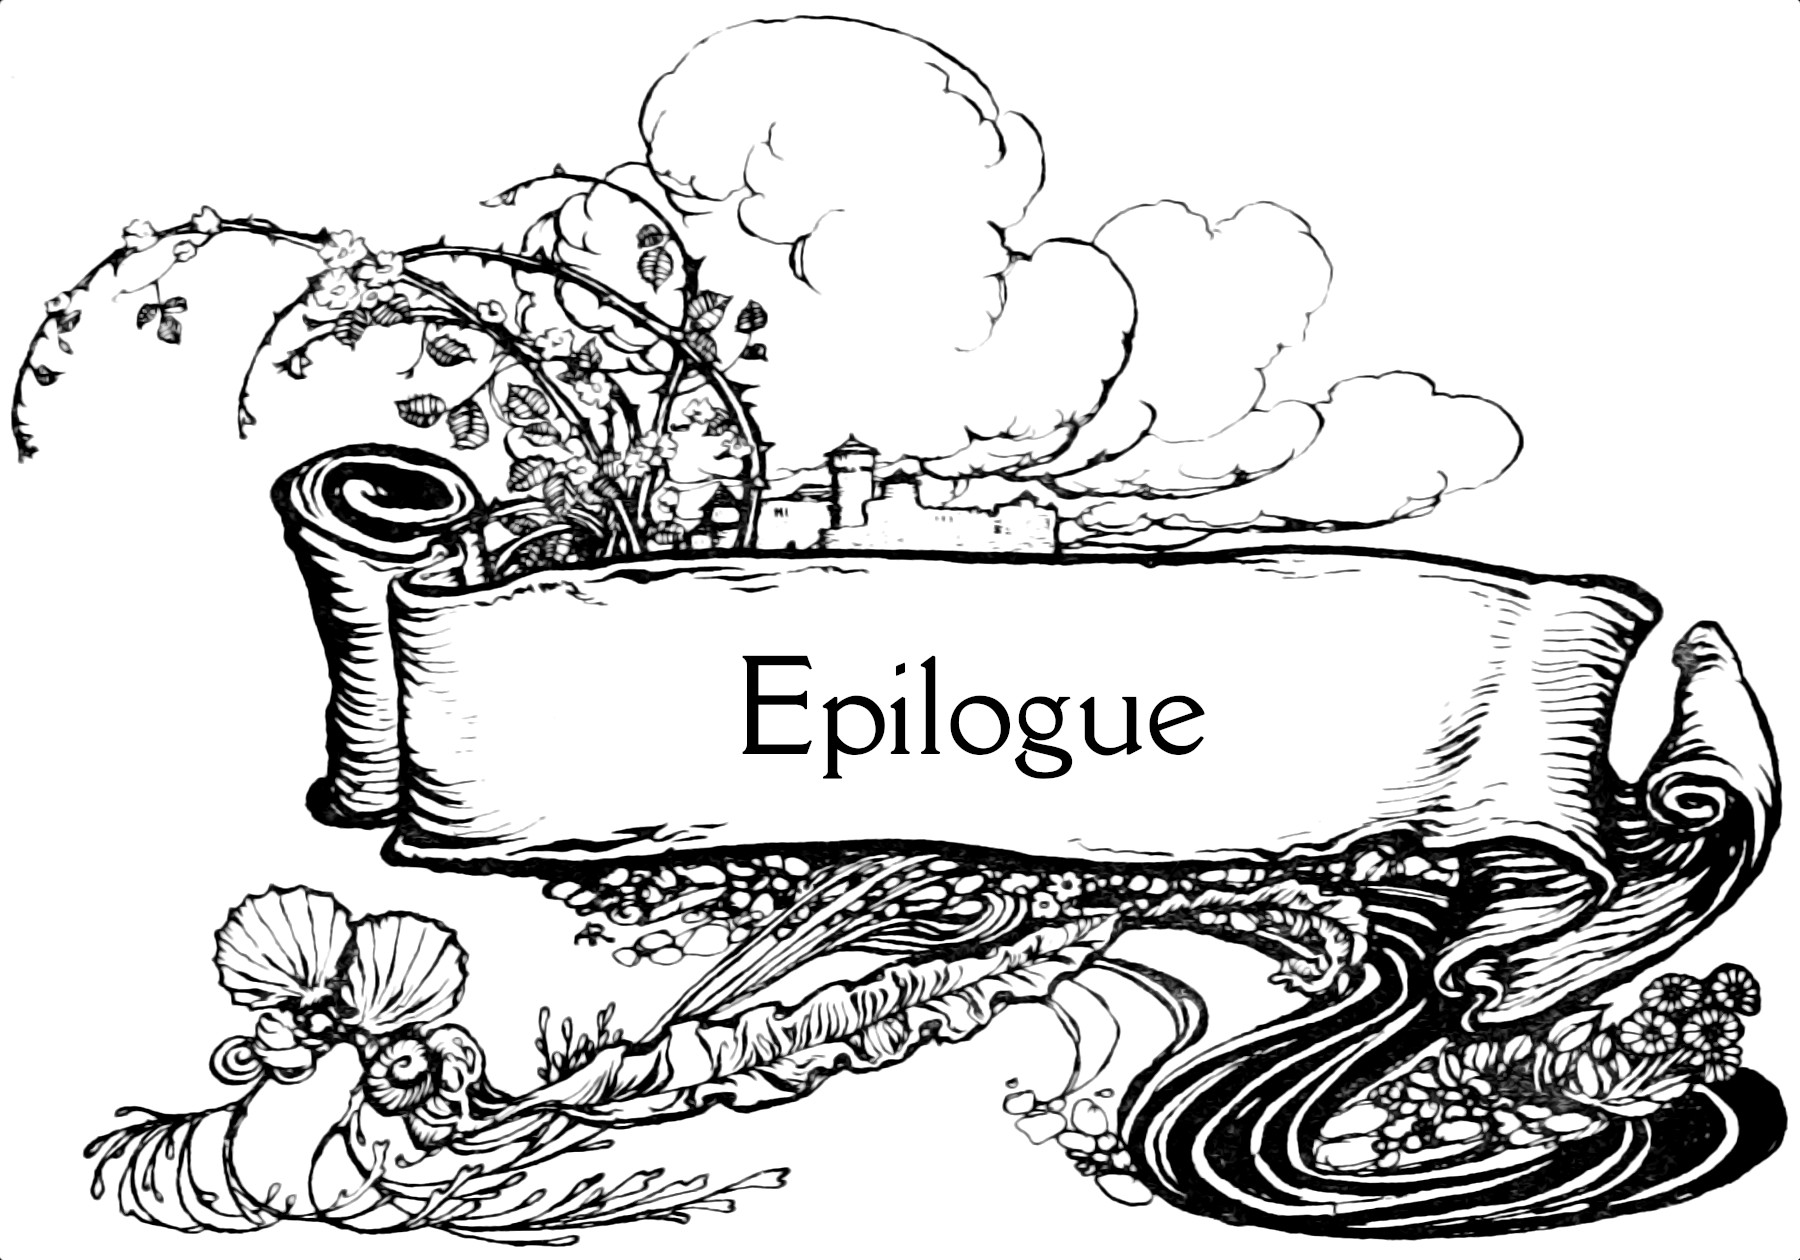
\includegraphics[width=.65\textwidth]{epihead}
	\end{figure}
\end{letter}
\begin{a4}
	\begin{figure}[t]
		\centering
		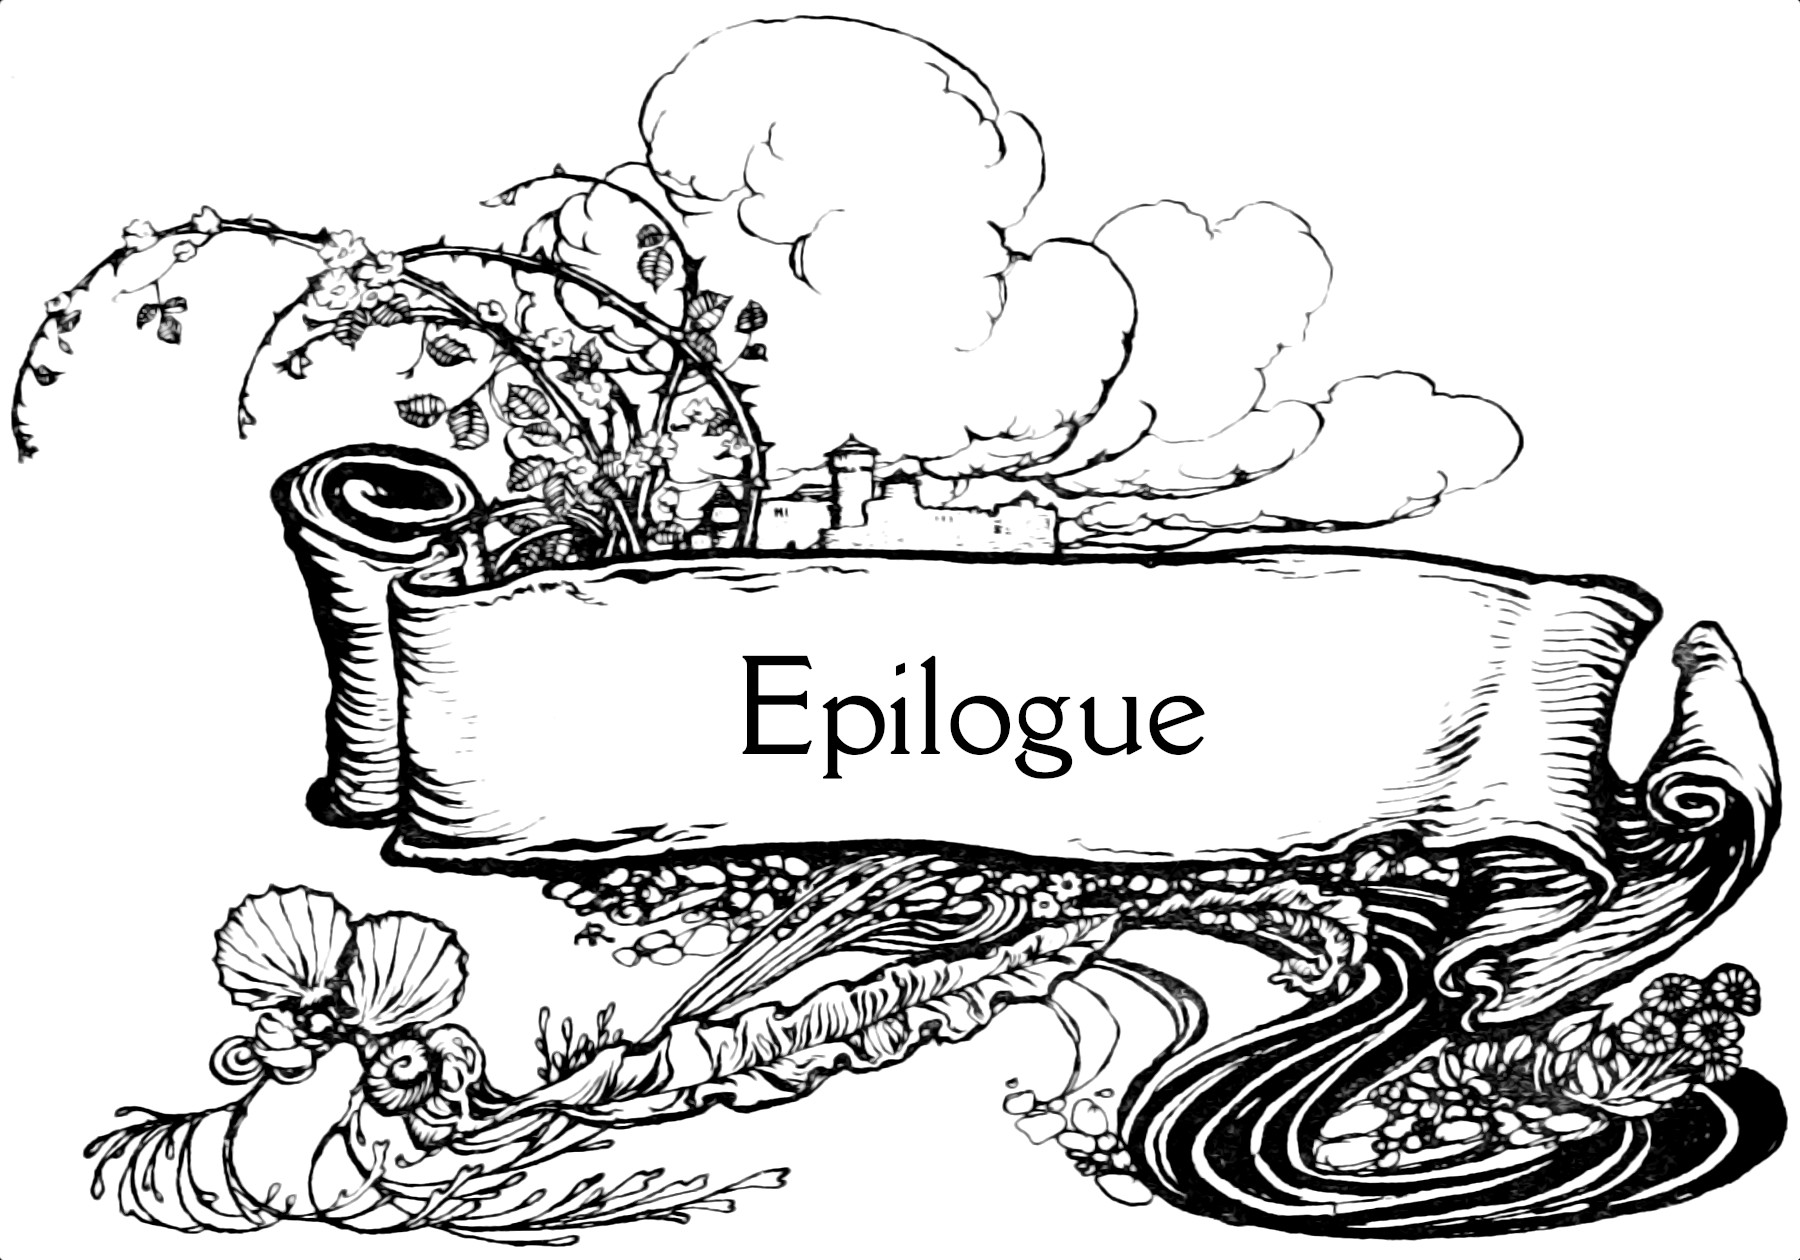
\includegraphics[width=.5\textwidth]{epihead}
	\end{figure}
\end{a4}

\vfill

\begin{verse_speech}[Prospero] 
Now my charms are all o'erthrown,\\
And what strength I have's mine own,\\
Which is most faint: now, 'tis true,\\
I must be here confined by you,\\
Or sent to Naples. Let me not,\\
Since I have my dukedom got\\
And pardon'd the deceiver, dwell\\
In this bare island by your spell;\\
But release me from my bands\\
With the help of your good hands:\\
Gentle breath of yours my sails\\
Must fill, or else my project fails,\\
Which was to please. Now I want\\
Spirits to enforce, art to enchant,\\
And my ending is despair,\\
Unless I be relieved by prayer,\\
Which pierces so that it assaults\\
Mercy itself and frees all faults.\\
As you from crimes would pardon'd be,\\
Let your indulgence set me free.
\end{verse_speech}
%\thispagestyle{plain}

\vfill